\chapter{Parallel Execution with MapReduce}

\section{Vertical and Horizontal Scaling}

Some important computer applications are so large that they would take
unacceptably long to execute on typical computers.  For
example, your personal computer is more than powerful enough
to balance your checkbook.  But what about a banking
application that tracks credit card usage in real time to
detect instances of fraud?  The sheer number of credit card
transactions make this application far too time-consuming for any
personal computer to handle.

Since these applications are important uses of computers,
computer scientists have come up with different ways of coping
with problems at large scale.  The traditional way is called
\textbf{vertical scaling}, and it consists of running the
application on a single, very powerful machine.

This is, of course, the easiest possible solution,
since the program is unchanged. But what happens as the
problems get bigger?  For example, the number of credit card
transactions increases over time.  Can a single computer, even
a very large one, keep up?  And if it can't, do you have to
upgrade by buying an even larger, more powerful (and more
expensive) computer?

\textbf{Horizontal scaling} offers an alternative.  Instead of
running the application in a single, large computer, with
horizontal scaling the application is split into smaller
chunks, and each chunk is run on a separate computer.
Ideally, the computers used are similar in almost all respects
to personal computers, so that the cost of an additional
machine is minimal.  This makes it more economical to scale the
hardware platform as the problems become larger.  Not
surprisingly, horizontal scaling has become the de facto
scalability solution for modern websites, including Google,
eBay, Amazon, and many others.

The problem with horizontal scaling, however, is that it is
not always easy to split your application into smaller
chunks.  In fact, this is particularly hard when the program
is written using traditional programming languages, such as
C++ or Java.  In those languages, the program is described as
a sequence of steps that the computer must take.  But that
becomes more difficult to do, as the number of computers
increases, because the programmer must also take into
consideration the interaction between the computers.

One of the advantages of the functional style of programming
that we have presented in this book is that there are no
interactions between different pieces of the code.  Instead,
everything is defined by mathematical functions, and it does
not matter where or when the functions are executed, since the
result is a matter of mathematical definition.

The engineers at Google were faced with one of the largest
scaling problems in the world, namely searching the entire
web.  To match the scale of this problem, they decided to use
the horizontal scaling approach.  Even though they use C++
internally, they invented and adopted a style of
programming called MapReduce, which is based on a functional
programming paradigm, very similar to the programming style
presented in this book.  Since Google's introduction,
MapReduce has been adopted in many other settings.  For
instance, the Apache Foundation implemented Hadoop, an
open-source implementation of MapReduce that you can freely
download to your computer.  Hadoop is widely used in industry
and academia.  Although we will not try to describe the full details of
Google's MapReduce or Apache's Hadoop implementation, we will
show you how the MapReduce framework simplifies the
development of programs that can scale horizontally by
focusing on just two operations.

\section{Introduction to MapReduce}

The MapReduce paradigm is applicable to problems that process
a dataset that can be described as a sequence of key/value
pairs.  Clearly, not all problems can be characterized in this
manner, but Google engineers recognized that many practical
problems do fit in this category.  Here are some examples.

\begin{itemize}
\item \textbf{Counting Words in a Document.}  The dataset, of
course, is the collection of words in the document.  It can be
organized as a list of word/count pairs, where the counts
are initially set to one.  Note that each word may have more
than one word/count pair initially.  The result of the
operation would be a list of word/count pairs where each word
appears only once.
\item \textbf{Finding Words that Link to a Webpage.}  The
purpose of this operation is to find the words that are used
most commonly to link to a particular page.  For example,
your name may be the most common phrase used to link into your
Facebook page.  Google uses this information to select which
pages to display for a particular search.  This problem, too,
can be implemented using MapReduce.  The dataset is the
(very large) collection of links on the Internet.  This can be
represented as a list of word/URL pairs, where the same word
may appear multiple times.  The solution will be a list of
URL/word pairs, where each URL will appear once, associated
only with the word that is used the most to link to it.
\item \textbf{Finding Extreme Values.}  For example, consider
an application that finds the record high and low temperature
for each state.  The initial dataset consists of a list of
city/temperature data.  There would be one record for each
city and each day, for as long as records are kept.  In fact,
there may be more than one record for a given data per day,
e.g., one record each hour.  Similarly, the output consists of
state/high or state/low records.
\end{itemize}

What all these applications have in common is that it is
possible to process each individual input record without
having to simultaneously examine all other records.  For
example, you can process the November 9, 2010 temperature
entry for Norman, OK without considering the May 3, 1932 entry
for Laramie, WY.  This enables horizontal scaling, because the
different entries can be processed in different machines.

However, these applications also show the need for combining
the entries for a specific key at a later time.  For example,
to find the low temperature record for Laramie, WY, it is
necessary to consider all entries for Laramie, WY at some
point.

The MapReduce paradigm makes it easy to implement programs
such as the above.  Processing is divided into two parts.  The
first part is the \texttt{map} function, which receives each
of the initial key/value pairs, one at a time, processes the
pair, and produces an arbitrary number of intermediate
key/value pairs.  These intermediate pairs use keys that may
or may not be completely different than the input keys.  In the
word counting example, the intermediate keys may be the same
as the input keys, namely the words that are being counted.
On the other hand, when looking for words that are used to
link to URLs, the input keys are the words, but the
intermediate keys are the URLs. The MapReduce framework leaves
this entirely up to you, and that is one of the reasons why
MapReduce is so widely applicable.

The second step is the \texttt{reduce} function, which
combines all the entries for each intermediate key and
produces zero or more final key/value pairs.  As before, the
final key/value pairs may use the same keys as the
intermediate or initial key/value pairs---or they may use
entirely different keys.

For example, consider the problem of counting words in a
document.  We can assume that the document has already been
read, and that it has been broken up into key/value pairs
where each key is a word and the value is always one.  For
instance, the Gettysburg address would be represented with the
list
\begin{itemize}
\item ( four . 1 )
\item ( score . 1 )
\item ( and . 1 )
\item ( seven . 1 )
\item ( years . 1 )
\item \dots
\item ( from . 1 )
\item ( the . 1 )
\item ( earth . 1 )
\end{itemize}
Here we use the notation ``( key . value )'' to denote a single
key/value pair.

Recall that the map function takes in an initial key and
value, and it should return zero or more intermediate
key/value pairs.  For the wordcount program, map should return
a single key/value pair, equal to the initial key and value.
\begin{displaymath}
map(k, v) = [ ( k . v ) ]
\end{displaymath}

The reduce function accepts an intermediate key and a list of
the values returned by map for that key.  It should return a
list of final key/value pairs.  In the case of wordcount,
reduce returns only one key/value pair, namely the key and the
sum of the counts in the list.
\begin{displaymath}
reduce(k, vs) = [ ( k . sumlist(vs) ) ]
\end{displaymath}
The function sumlist, which adds all the elements of its
input, is not defined, but you should be able to fill in the
details.

The magic of MapReduce is now apparent.  You only need to
define the map and reduce functions as above.  The MapReduce
framework takes care of running the program in a single
computer, or in a cluster of hundreds of computers, depending
on the size of the problem.

What, exactly, does the MapReduce framework do?  First, it
takes the initial key/value pairs and splits them across many
different machines.  On each machine, it calls the map
function on each of the key/value pairs that is assigned to
that machine.  As it does this, it combines the intermediate
key/value pairs returned by each call to map into a single
list.  The lists from all of the machines are then combined.

On first thought, it may appear that all of the intermediate
lists need to be combined.  But actually, this is not the
case.  The reason is that the reduce function needs to see an
intermediate key and all the values associated with that key.
But different intermediate keys are independent, so they can
be processed by different machines.  What this means is that
it is necessary to collect all of the intermediate values for
each of the intermediate keys.  This can help to distribute
the calls to reduce across the entire cluster of machines
running MapReduce.

Once all the values for a given intermediate key are
collected, the MapReduce framework can call the reduce
function on that intermediate key.  The result is a list of
final key/value pairs, and MapReduce collects all these
results and returns them as the final answer.

As you can see, MapReduce is doing all of the work
related to distributing the program across multiple machines.
That is exactly the way it was designed, and it explains its
growing popularity.  You can develop a MapReduce program on
your local computer, modifying it until it behaves exactly as
you want it to on a small set of data.  Then, you can submit
the program to a large MapReduce cluster and run it on the
entire data set.

\section{Data Mining with MapReduce}

Now that we have seen the basics of MapReduce, it is time to consider
a larger example, something that illustrates how MapReduce is being
used in practice.  The application we will look at is a recommendation
engine, a piece of code that is used to recommend new things to you based
on other things you like.  For example, when you visit a product page at
Amazon.com, you will likely see a section called ``Customers Who Bought
This Item Also Bought'' that recommends related items.  Based on your
past purchases and browsing habits, Amazon.com also builds a web page
full of recommended items that is customized for you.  How can Amazon.com
do this?

The answer is easy to understand after we break the problem down into
two components.  First, Amazon.com needs to finds \textit{customers like
you}.  In the case of a single product, this means other customers who
have bought this product.  In the more general sense, used to create custom
recommendation lists for you, it means other customers who have bought many
of the same items that you have purchased in the past.  Once the group of
customers like you is identified, the rest of the problem is easy.  Each
person in that group has made some purchases, so it is only necessary to
find the most popular items in that group.

Finding the most popular items is essentially the same as counting words
in a document.
Amazon.com keeps a history of all the purchases that each of its
customers have made.  To process this list with MapReduce, think of it as
consisting of entries of the form customer/item, meaning that the given
customer bought that particular item.  Similar to the wordcount program,
the map operation produces intermediate entries of the type item/1, meaning
the given item was bought (once).  Such an entry should be generated for
each purchased \textit{made by a customer in the reference group.}  That is,
the map operation filters out the purchases made by customers who are
not like you.  The reduce operation is identical to wordcount's, but this
time it counts the number of purchases for each item.  The only remaining
detail is to consider the results of the reduce operation and select the
items that were purchased most often.

Unfortunately, that leaves the first problem, namely finding the group of
customers who are most like you.  This is the most critical aspect for
generating useful recommendations.  For instance, if you have only ever
purchased gardening books from Amazon,com, you are likely to ignore a
recommendation engine that alerts you to the latest novel in a long-running,
young adult, vampire series.  Worse, you may start thinking of the recommendations
as unwarranted spam.

How can Amazon.com find customers just like you?  Imagine, first of all, that
you have rated all the purchases you have made, giving each item a grade between
0 (hated it) and 5 (loved it).  To keep things simple, imagine that Amazon.com
sells only two items.  Then your ratings for these items can be expressed as
a pair of numbers, say (2, 0).  Now suppose that other customers have similarly
rated the items.  The customers who are most like you are precisely the ones
whose ratings are close to your score or (2, 0).  Effectively, your purchase
history is represented by a point at coordinate (2, 0), and the customers who
are most like you are have purchase histories that correspond to nearby points.

Of course, Amazon.com sells many more than two items!  And neither you nor any
of Amazon.com's other customers are likely to have rated even a fraction of them.
But the principle stays the same.  Instead of using pairs to represent your
ratings, we need many more coordinates---as many as Amazon.com has products.
But this is still just a point, albeit in a space with many dimensions.  And the
customers most like you will still be represented by points close to yours.

A remaining complication is that customers do not always explicitly rate the
items they like, but this can be easily resolved by using implicit ratings.
For example, if you buy an item, we can give it a rating of 4, unless you
explicitly change it.  And any product that you have never even looked at
can be given a rating of 0.

So the problem is to find which points in this huge dimensional space are near
your own.  It is actually more useful to think of this a little differently.
Instead of finding points near yours, think in terms of finding groups of
points that are clustered together.  One cluster, for example, may consist of
avid gardeners, while another includes fans of young adult, vampiric fiction.

In general, finding clusters in a large dataset is a very complicated problem.
But there are some useful approximations.  For example, suppose that you expect
to find 10 clusters.  You could try to find them as follows:
\begin{enumerate}
	\item Initially, guess at the location of each cluster.  The guess can consist
		of the center point of each alleged cluster.
	\item For each point in the dataset, decide which cluster center is nearest
		to the point.  Split the points into clusters so that each point is
		in the cluster determined by the nearest center point.
	\item Next, recalculate each cluster's center point by averaging all the
		points that were assigned to that cluster.
	\item Repeat the previous two steps as many times as necessary to find the
		clusters.
\end{enumerate}
The middle two steps can be implemented using MapReduce.  The map operation can
assign points to clusters, while the reduce function can computes the new center
point of each cluster.  Note that if we know the center points, it is a trivial
matter to determine which cluster you belong to.  And once we know that, we can
determine, as we did before, which products are relevant to customers in your
cluster.

We have to be a little careful with the definition of the map and reduce functions.
In the earlier examples, the map function only had two arguments, a key and an
associated value.  But in this case, the map functions needs a purchase history (i.e.,
a point that represents an individual customer) and the current cluster center
points.  These center points should be the same for all purchase histories, so
they should not be included in either the key or the value.  Instead, we add an
argument to the map function as follows.
\begin{displaymath}
map(hist, v, centers) = [ ( closest\_center(hist, centers) . hist ) ]
\end{displaymath}
As you can see, the result of a map operation is an intermediate key/value pair, where the key
identifies a specific center point, and the value is the point representing the
current history.

The MapReduce framework will collect all the intermediate values and call the reduce
operation once for each key.  So the reduce operation sees all the points in each
cluster, and it can compute the new center point of the cluster by averaging the points
in the list.  Although reduce does not need to see the original center points, we pass
these to the reduce function to keep the symmetry with the map operation.
\begin{eqnarray*}
	\begin{array}{l@{}l}
		reduce(&cluster, \\
			   &points, \\
			   &centers)
	\end{array} &=& [ ( cluster . average(points) ) ] \\
average(points) &=& avg\_aux(points, (0,0), 0) \\
\begin{array}{l@{}l}
	avg\_aux(&points, \\
				 &sum, \\
				 &count)
\end{array} &=&
	\left\{
		\begin{array}{l@{}ll}
    		\multicolumn{2}{l}{sum / count,}  & \mbox{if } points = [] \\
    		avg\_aux(& rest(points),          & \mbox{otherwise} \\
					 & sum+first(points),     & \\
					 & count+0),              & \\
		\end{array}
	\right.
\end{eqnarray*}
The auxiliary functions average and avg\_aux are used to compute the new center point
of the cluster.  Notice that the addition and division operations are adding points,
not just numbers.

The result of the reduce operation is the new list of center points.  This should be
in the same format as the initial guess.  What this means is that the output of the
reduce operation can be passed back as the initial guess for subsequent passes of the
map step.  This allows us to execute as many map and reduce operations as necessary
to find the clusters, as illustrated in Figure~\ref{iterative-map-reduce}.

\begin{figure}
	\begin{center}
		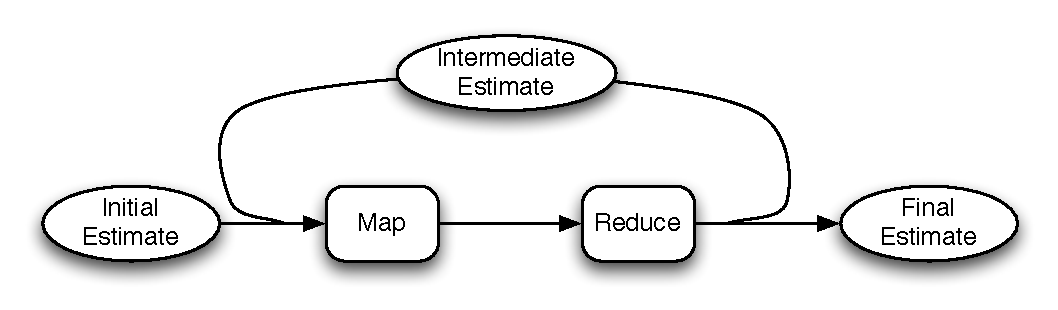
\includegraphics[scale=0.7]{images/iterative-map-reduce}
	\end{center}
	\caption{Iterative Map Reduce Operation}
	\label{iterative-map-reduce}
\end{figure}

\section{Summary}

Some problems are too large to solve on a single, conventional machine.  That leaves us
with two options.  We can either get a large machine, e.g., a supercomputer, or we can
break the problem down into many tasks and execute each task on a separate computer.

The first approach, vertical scaling, is limited by the size of the largest computer that
we can afford.  It is also difficult to use in practice, because as the problem grows,
e.g., as a website attracts a growing number of users, several scaling steps may be
necessary, and each step requires an expensive migration to a more capable computer.

The alternative approach, horizontal scaling, offers the promise of virtually unlimited
scalability and a gradual increase in the cost of the solution as the problem size grows.
But it is much more difficult to write programs that are split across multiple machines.
Also, this solution only applies to problems that can be reasonably split.  Such problems
usually involve a large data set, and portions of this data can be processed independently.

Based on equational programming, MapReduce is a framework that makes it easy to write
programs that can be distributed across a large number of computers.  MapReduce programs are
organized around two functions.  The Map function applies to each of the input values, and
it generates an intermediate result.  The intermediate results are subsequently combined using
the Reduce function.  If the results generated by the Reduce function are in the same format
as the input to the Map function, multiple MapReduce passes can be performed.  This is useful
in programs that estimate optimal results by refining an initial estimate, such as programs that
find clusters in a large dataset.

%%% Local Variables:
%%% mode: latex
%%% TeX-master: "book"
%%% End:
